\documentclass[11pt, a4paper,oneside,chapterprefix=false]{scrbook}

\usepackage{a4wide}
\usepackage{times}
\usepackage{helvet}   % sets sans serif font

\usepackage{amsmath,amssymb,amsthm}

\usepackage{graphicx}
\usepackage{subfigure}  
\usepackage{fancybox} % for shadowed or double bordered boxes
\usepackage{fancyhdr}
\usepackage[dvipsnames]{xcolor}
\usepackage{rotating}

\usepackage{hyperref}
\hypersetup{
    colorlinks=true,
    linkcolor=blue,
    filecolor=magenta,      
    urlcolor=cyan,
}

\DeclareGraphicsExtensions{.pdf, .jpg, .png}
\DeclareOldFontCommand{\sf}{\normalfont\sffamily}{\mathsf}

%% macros
 \def\mathbi#1{\textbf{\em #1}}
 
% commands
\newcommand{\Adjoint}{\mbox{\rm Adj}}
\newcommand{\Area}{\mbox{\rm Area}}
\newcommand{\ACos}{{\mbox{\rm Cos}^{-1}}}
\newcommand{\ASin}{{\mbox{\rm Sin}^{-1}}}
\newcommand{\ATan}{{\mbox{\rm atan2}}}
\newcommand{\Code}[1]{{\tt #1}}
\newcommand{\Complex}{\mbox{\bf C}}
\newcommand{\Cross}{{\mbox{\rm Cross}}}
\newcommand{\Mydddot}[1]{\mbox{\shortstack{$.$\hspace*{-1pt}$.$\hspace*{-1pt}$.$\\$#1$}}}
\newcommand{\Degree}{\mbox{\rm degree}}
\newcommand{\Diag}{\mbox{\rm Diag}}
\newcommand{\Dim}{\mbox{\rm dim}}
\newcommand{\Dist}{\mbox{\rm Distance}}
\newcommand{\IntTwo}{\int\!\!\int}
\newcommand{\IntThree}{\int\!\!\int\! \!\int}
\newcommand{\Kernel}{\mbox{\rm kernel}}
\newcommand{\Kross}{\mbox{\rm Kross}}
\newcommand{\Grad}{\nabla}
\newcommand{\Perp}{\mbox{\rm Perp}}
\newcommand{\Point}[1]{{\cal #1}}
\newcommand{\Rank}{\mbox{\rm rank}}
\newcommand{\Range}{\mbox{\rm range}}
\newcommand{\Real}{{\mbox{\rm I}\hspace*{-2pt}\mbox{\rm R}}}
\newcommand{\RealSbt}{{\mbox{\rm\scriptsize I}\hspace*{-2pt}\mbox{\rm\scriptsize R}}}
\newcommand{\Res}{\mbox{\rm resultant}}
\newcommand{\Sbt}[1]{{\mbox{\rm\scriptsize #1}}}
\newcommand{\MySign}{\mbox{\rm Sign}}
\newcommand{\SignSBT}{\mbox{\rm\scriptsize Sign}}
\newcommand{\Skew}{\mbox{\rm Skew}}
\newcommand{\Span}{\mbox{\rm Span}}
\newcommand{\SqrDist}{\mbox{\rm Distance$^2$}}
\newcommand{\Trace}{\mbox{\rm Trace}}
\newcommand{\TRN}{{\mbox{\rm\scriptsize T}}}
\newcommand{\Vector}[1]{\mbox{\bf #1}}
\newcommand{\VectorM}[1]{\mbox{\boldmath $#1$}}
\newcommand{\Volume}{\mbox{\rm Volume}}

\newcommand{\IVec}{\mbox{\boldmath $\imath$}}
\newcommand{\JVec}{\mbox{\boldmath $\jmath$}}
\newcommand{\KVec}{\mbox{\boldmath $k$}}
\newcommand{\LVec}{\mbox{\boldmath $\ell$}}
\newcommand{\RMat}{{\cal R}}
\newcommand{\QMat}{{\cal Q}}
\newcommand{\QCMat}{\overline{\cal Q}}

\newcommand{\Lerp}{\mbox{\rm lerp}}
\newcommand{\Slerp}{\mbox{\rm slerp}}
\newcommand{\Quad}{\mbox{\rm quad}}
\newcommand{\Squad}{\mbox{\rm squad}}

\newcommand{\ODer}[2]{\frac{d #1}{d #2}}
\newcommand{\ODerT}[2]{\frac{d^2 #1}{d {#2}^2}}
\newcommand{\ODerM}[3]{\frac{d #1}{d #2 \, d #3}}
\newcommand{\PDer}[2]{\frac{\partial #1}{\partial #2}}
\newcommand{\PDerT}[2]{\frac{\partial^2 #1}{\partial {#2}^2}}
\newcommand{\PDerM}[3]{\frac{\partial^2 #1}{\partial #2 \, \partial #3}}

% mass density symbol
\newcommand{\Den}{\delta}

% environments
\newenvironment{BArray}[1]{\left\{ \begin{array}{#1}}{\end{array} \right\}}
\newenvironment{Combin}{\left( \begin{array}{c}}{\end{array} \right)}
\newenvironment{Matrix}[1]{\left[ \begin{array}{#1}}{\end{array} \right]}


\let\mbf=\mathbf
\let\mvec=\mathbf
\let\mcal=\mathcal
\let\mfunc=\mathrm

%\def\R{\mbox{\ensuremath{\mathrm{I\!R}}}}
\newcommand{\R}{\ensuremath{\mathbb{R}}}
\newcommand{\N}{\ensuremath{\mathbb{N}}}
\newcommand{\Z}{\ensuremath{\mathbb{Z}}}
\newcommand{\C}{\ensuremath{\mathbb{C}}}

\newcommand{\of}[1]{\left( #1 \right)}
\newcommand{\abs}[1]{\left| #1 \right|}
\newcommand{\norm}[1]{\left\Vert {#1} \right\Vert}
\newcommand{\gradient}[1]{\nabla{\!}_{#1}{\,}}
\newcommand{\twovec}[2]{\left( #1 \atop #2 \right)}
\newcommand{\threevec}[3]{\left(\begin{array}{c}#1\\#2\\#3\end{array}\right)}
\newcommand{\fourvec}[4]{\left(\begin{array}{c}#1\\#2\\#3\\#4\end{array}\right)}

\newcommand{\refsec}[1]{Section~\ref{sec:#1}}
\newcommand{\reffig}[1]{Fig.~\ref{fig:#1}}
\newcommand{\reftab}[1]{Tab.~\ref{tab:#1}}
\newcommand{\refeq}[1]{Eq.~(\ref{eq:#1})}

%\newcommand{\R}{\hspace*{0.1ex}{\sf I} \hspace{-0.3ex}{\sf R}}

%6.5
\newcommand{\eps}{\mbox{$\epsilon$}}
\newcommand{\dmin}{\mbox{$d_{\min}$}}
\newcommand{\dmax}{\mbox{$d_{\max}$}}
\newcommand{\dminmax}{\mbox{$[\dmin,\dmax]$}}

%4.2:
\def\M{\mathcal{M}}
\def\n{\mathbi{n}}
\def\p{\mathbi{p}}
\def\q{\mathbi{q}}
\def\x{\mathbi{x}}
\def\tp{^{\mathsf{T}}}

\let\vec=\mathbi%
\let\mat=\mathbf%
\let\set= \mathcal%

% Taken from (and slightly modified): http://stackoverflow.com/questions/741985/latex-source-code-listing-like-in-professional-books

\usepackage{listings}
\usepackage{courier}
\usepackage{color}
\definecolor{lightgray}{gray}{0.9}
\definecolor{commentgreen}{rgb}{0.2,0.56,0.2}
 \lstset{
         basicstyle=\footnotesize\ttfamily, % Standardschrift
         numbers=left,               % Ort der Zeilennummern
         numberstyle=\tiny,          % Stil der Zeilennummern
         %stepnumber=2,               % Abstand zwischen den Zeilennummern
         numbersep=5pt,              % Abstand der Nummern zum Text
         tabsize=2,                  % Groesse von Tabs
         extendedchars=true,         %
         breaklines=true,            % Zeilen werden Umgebrochen
         keywordstyle=\color{red},
                frame=b,         
          keywordstyle=[1]\textbf,    % Stil der Keywords
         keywordstyle=[2]\textbf,    %
         keywordstyle=[3]\textbf,    %
         keywordstyle=[4]\textbf,   %\sqrt{\sqrt{}} %
         stringstyle=\color{blue}\ttfamily, % Farbe der String
         showspaces=false,           % Leerzeichen anzeigen ?
         showtabs=false,             % Tabs anzeigen ?
         xleftmargin=17pt,
         framexleftmargin=17pt,
         framexrightmargin=5pt,
         framexbottommargin=4pt,
         backgroundcolor=\color{lightgray},
         showstringspaces=false,      % Leerzeichen in Strings anzeigen ?
         commentstyle=\color{commentgreen}
 }
 \lstloadlanguages{% Check Dokumentation for further languages ...
         %[Visual]Basic
         %Pascal
         %C
		PHP, 
         C++
         %XML
         %HTML
         %Java
 }
    %\DeclareCaptionFont{blue}{\color{blue}} 

  %\captionsetup[lstlisting]{singlelinecheck=false, labelfont={blue}, textfont={blue}}
  \usepackage{caption}
\DeclareCaptionFont{white}{\color{white}}
\DeclareCaptionFormat{listing}{\colorbox[cmyk]{0.43, 0.35, 0.35,0.01}{\parbox{\textwidth}{\hspace{15pt}#1#2#3}}}
\captionsetup[lstlisting]{format=listing,labelfont=white,textfont=white, singlelinecheck=false, margin=0pt, font={bf,footnotesize}}

\usepackage{color}
\definecolor{RED}{rgb}{1,0,0}
\definecolor{GREEN}{rgb}{0,0.7,0}
\definecolor{BLUE}{rgb}{0,0,1}
\newcommand{\FIXME}[1]{{\color{RED}{\textbf{FIX}: #1}}}

\addtolength{\textheight}{2.0cm}
\addtolength{\voffset}{-1cm}
\addtolength{\textwidth}{1.8cm}
\addtolength{\hoffset}{-.9cm}

\widowpenalty=10000
\clubpenalty=10000

\newcommand{\todo}[1]{}
\renewcommand{\todo}[1]{{\color{red} TODO: {#1}}}


\lstdefinelanguage{JavaScript2}{
  keywords={typeof, new, true, false, catch, function, return, null, catch, switch, var, if, in, while, do, else, case, break, for, forEach},
  keywordstyle=\color{orange}\bfseries,
  ndkeywords={class, export, boolean, throw, implements, import, this},
  ndkeywordstyle=\color{darkgray}\bfseries,
  identifierstyle=\color{black},
  sensitive=false,
  comment=[l]{//},
  morecomment=[s]{/*}{*/},
  commentstyle=\color{purple}\ttfamily,
  stringstyle=\color{ForestGreen}\ttfamily,
  morestring=[b]',
  morestring=[b]"
}

\begin{document}

\frontmatter
%\maketitle %automatic version
% --- selfmade version ----
\begin{titlepage}
	\setlength{\parindent}{0cm}
	\addtolength{\textheight}{1.0cm}

	\vspace{0.5cm}
	\Huge
	{\textbf{A visualization of biodiversity through time\\ }}

	\vfill \vfill \vfill
	%\begin{center}
	%\includegraphics*[width=0.8\textwidth]{images/title.jpg}
    %\end{center}
	\vfill
	\sf \Large
	Master Thesis \\
	\today \\[0.5cm]
	\large
	by Wuxing Dong, 18-946-038

	\vfill \vfill \vfill
	\begin{minipage}[b]{0.5\textwidth}
	Supervisors: \\
	Prof. Dr. Renato Pajarola \\
	Gaudenz Halter \\
	\end{minipage}
	%
	\begin{minipage}[b]{0.5\textwidth} \raggedleft
	Visualization and MultiMedia Lab \\
	Department of Informatics \\
	University of Z{\"u}rich
	\end{minipage}

	\vfill
	\hrule
	\vspace{0.5cm}
	\includegraphics*[width=0.3\textwidth]{figures/cover/uzh_logo} \hfill
	\includegraphics*[width=0.3\textwidth]{figures/cover/vmml_logo}
\end{titlepage}
%%

%=====================================================================

%=====================================================================
\chapter{Abstract} \label{chp:abstract}
%=====================================================================

The increasing size and dimensionality of datasets in the humanities pose new challenges to scholars working with them, including how to establish an overview over the dataset, how to establish new hypotheses and how to test them. Material, pattern, and texture usage in moving image is an attractive example of such multi-dimensional datasets in film studies, as an almost infinite number of combinations thereof are possible.\\ 
This thesis proposes interactive data visualization and exploration of film features as a solution to assist film researchers in the investigation of relationships between material, pattern, textures, and a wide range of qualitative analysis labels in a large film database. Using an array of visual components in combination with exhaustive computational methods and an interactive user-interface, the proposed solutions show to be effective in conveying the global and local structure of the dataset as well as the relationship between different feature groups of features. Finally, the resulting visualization tool is embedded into the well-established research framework of the FilmColors project.


%=====================================================================

\tableofcontents

\mainmatter


%=====================================================================
\chapter{Introduction} \label{chp:introduction}
%=====================================================================

\section{Effective visualization of data} \label{sec:one}
In the time of the information age, the Internet has become a primary source to educate ourselves about the world. It is therefore a great opportunity for the scientific community to take advantage of the web and create high quality products to communicate their findings and ideas to the non-experts and general public. Textbook-styled verbal explanations can be rigorous, however, they easily become tedious and are already made available by school and college education. Videos are based on visual learning, quick to absorb, yet there is no engagement with the viewers. An interactive data visualization can provide an excellent way for users to understand scientific concepts. New knowledge is conveyed by direct visual impact that easily draw attention, and insights can be formed by actively exploring the data and observing the response of the presentation due to the users' own actions. This learn-by-doing strategy can consolidate the new knowledge. \\

Although graphics plays a major role to deliver scientific messages, there is a lack of formal theory on producing good graphics, and domain experts tend to rely on practical experiences that are guided by certain design principles. Increasing amount of studies have focused on concluding such principles. Chen and colleagues have summarized that three main aspects to pay attention to in a visualization project are its contents, the relevance in the context of the larger whole as well as the forms and aesthetics (construction). Similarly, McCandless argued that a good visualization requires integrity of information, interestingness of story (concept), usefulness of goal and beauty of the visual form.\\

Before embarking on the production of a visualization, one should note the characteristics of human visual perception to improve the design strategies in practice. Cognitive psychological studies aimed at examining human visual attention by exposing users to certain visual processing tasks. The results of those studies suggested some guidelines for more effective visualization. When the visual features of a certain type of data is expected or previously known, the accuracy and speed of visual perception is drastically improved. Therefore, a visual feature should be assigned to the same data dimension, or type of data. It is also important to note that attention is limited and selective, therefore the amount and diversity of information should be kept within the limits of cognitive load. When many categories of data are present, compromises are needed to retain graphics complexity and only demonstrate a few number of categories at a time. \\

Through early years of research on how images are analyzed visually, it has been found that detailed vision is only achievable by actively focusing on small portion of the visual field. However, a few visual features, such as colors and curvatures, are subjected to preattentive processing, which can be effortlessly and rapidly detected by low-level visual processes. Colors is thus a powerful method in graphics. It can encode extra layers of information, and serves a leading factor to make a visualization memorable. Three major schemes for using colors are sequential, diverging and qualitative. A sequential scheme relates increasing value of the data to the intensity of the color, while using only one or two hues. In diverging scheme, two extremes are shown by two sequential schemes, and the middle or neutral value corresponds to a white or neutral color. The qualitative scheme uses a variety of distinguishable colors to represent data belonging to distinct categories. It is a good practice to choose color schemes that are distinguishable enough, such that minimal information is lost when converted into a gray scale. In addition, when a range of colors are used together, reducing the opacity of certain or all colors avoids overwhelming visual impact to the viewers. \\

Design principles have also been examined and summarized by different studies. The design process should be guided by the core messages to deliver. It is important to first prioritize what information to show, envision the final result, and then choose appropriate geometries that fulfill the objectives. Geometries are the forms in which data is illustrated, and the majority of them can be categorized into amounts, compositions, distributions or relationships. Often, different geometries can be considered on the same data, however, the most efficient geometry should be of high data-ink ratio, which is the ratio between the amount of ink allocated on the actual data to the total amount of ink used in a figure. While a high data-ink ratio indicates high efficiency, it is also important for a visualization to be simple, self-explanatory  and straight to the points, such that the viewers are not overwhelmed with too much information. \\


\section{Background on biodiversity and tectonic change} \label{sec: two}
The data this thesis chooses to visualize is biodiversity through earth history. Considering various pressing environmental issues nowadays, it is important to raise the awareness of the general public on how different forms of life came to exist and change during the course of earth history. Climate change has become a non-negligible factor influencing on our daily life and the future of human society. Recently, the world sees increasing amount of extreme weather conditions, causing significant losses in human lives and properties. The ecosystem is also under threat of a mass extinction event, after which 90\% of all species are expected to disappear, and its leading cause is considered to be human activity. 
By understanding the history of life through simple and interesting visualizations, viewers could appreciate the inseparable relationship with our environment, and be more promoted to act in a more environmentally-friendly and sustainable manner.

\subsection{Biodiversity as a result of evolution} \label{subsec: one}
\begin{figure}[h]
	\centering
	\subfigure[John Gould's sketches of the various beak shapes of the Galapagos finches as a result of evolution. ]{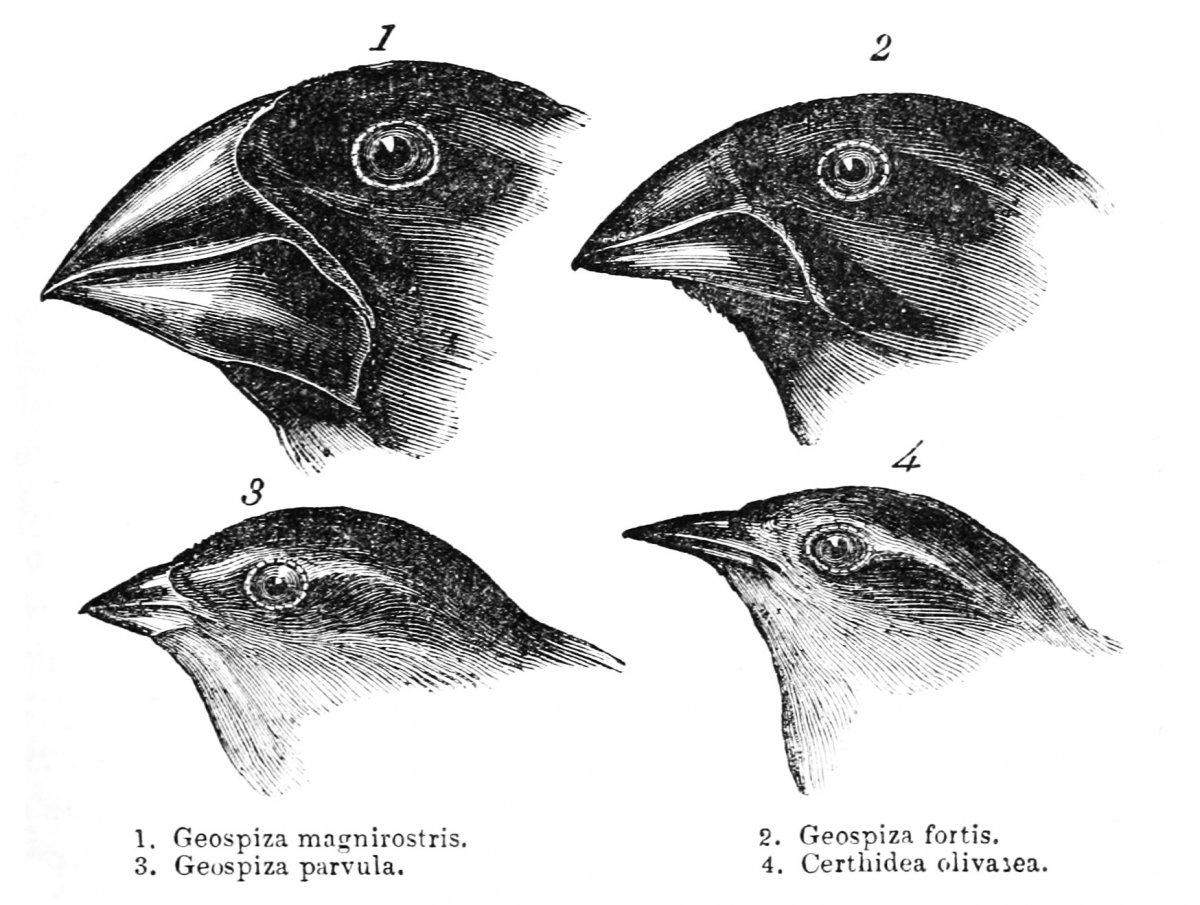
\includegraphics[width=0.45\textwidth]{figures/introduction/finches}\label{fig:finches}} 
	\hfill
	\subfigure[Biodiversity during Phanerozoic experiences non linear change with mass extinction events. ]{\includegraphics[width=0.45\textwidth]{figures/introduction/phanerozoic_biodiversity}\label{fig:phanerozoic_biodiversity}} 
	\label{fig:evolution}
\end{figure}
Current views on the process of species formation is based on modern evolution theory originated from Darwin's work. To summarize briefly, all forms of life are argued to share a common ancestor, which diversified over the course of evolution to form the current tree of life. An organism's genomic information is encoded in DNA or RNA, which is replicated over generations. However, recombination and random mutation events occur during the replication process, resulting in genetic variations, which in turn causes difference in phenotype, the observable traits of organisms. Individuals with traits that are more suitable to their particular environment are more likely to survive and pass their genes to their offspring, comparing to those that are poorly adapted to the environment. This process is termed natural selection. A classic example of evolution is the adaptive radiation of finches on the Galapagos islands. The beak shapes of the finches on different islands diversified to specialize on obtaining the dominant type of food on different islands. Over generations, species evolve as a consequence of the change in the prevalence of advantageous genes. Finally, a new species is formed during the process of speciation. It occurs when enough genetic variations are accumulated between the original population and the descendant population, such that organisms from the two groups are not capable of producing fertile offspring, namely, the two groups have reproductive isolation. \\

It is believed that life emerged from 3.5 billion years ago. The past 540 million years ago (the Phanerozoic Eon) sees rapid development and diversification of life. Throughout evolutionary history, there are records of drastic changes in biodiversity occurring in a relatively short period of time. Radiations are rapid increase in biodiversity. An example is the Cambrian explosion, during which most phylums of multi-cellular organisms appeared. On the contrary, biodiversity experiences rapid decline during mass extinction periods. There is evidence of five mass extinction periods, one of which occurred in Cretaceous and Tertiary, when the dinasours were exterminated and mammals thrived due to their selective advantage given by their fur in the cooling environments. These periods of radiation or extinction are caused by special events, plate motions, as well as change in climate, such as temperature and oxygen level. \\

\subsection{Tectonic shift as a driver of biodiversity change} \label{subsec: two}
The earth crust is composed of a number of tectonic plates undergoing constant changes. The hear generated from the interior of the planet causes the movement of the plates, as a result, earth appears very differently throughout millions of years of history. The plate motion results in new landscapes and new continents, affecting the inhabitants of lives. For instance, the current continents are thought to belong to one super continent called Pangaea, and gradually drifted away from each other since 175 million years ago. \\

As the continents separated, populations from the same species are geographically isolated into their particular environments that is created from the plate motion. Since organisms are under constant selective pressure from the environment, new species are formed in the newly created environments. An example is the distribution of ratite as a result of tectonic movement. 

\section{Source of data} \label{sec:three}
\emph{The fossil}\\
The biodiversity of ancient time periods is represented by fossil records. For this purpose, we use paleodb, which contains 1.3 million occurrences of fossil records. Each record has its unique ID, identified taxonomy, estimated maximal and minimal time (in million years) to today, and their coordinates. \\

\noindent \emph{The tree}\\
All identified species are classified in taxonomy, following the hierarchy of domain, kingdom, phylum, class, order, family, genus and species. Therefore, it can be naturally organized into a tree structure. Conveniently, for each fossil record in PBDB dataset, the names on each rank of the taxonomy is available. The highest taxonomy rank in the PBDB dataset is kingdom, namely the kingdom of Animalia (animal) and Plantae (plants). Since the two kingdoms are under the domain of Eukaryota, a rooted tree of life can be generated from the taxonomy information of all fossil record.\\

\noindent \emph{The map}\\
The geological information is provided by Matthew and colleagues, who traced the coastlines of the continents from 410 million years ago until the current world. 

\section{Aim of the thesis}
This thesis aims at building a web application that visualizes the change in biodiversity through the course of earth history. In the final product, users can view a customizable tree of life during a selected time period under a selected taxonomy. In the meantime, the fossil records belonging to the given tree of life is shown on the map, whose coastlines correspond to that of the selected epoch in ancient time. 

\section{Thesis structure}
Chapter one introduces the topic of data visualization and domain specific background information, and it claims the goal of the thesis. Chapter two analyzes some related work, indicating what could be learned and improved for the visualization to be built. Chapter three outlines the problems to be solved at each stage for building the web application. Chapter four discuses the technical solutions for data processing and web development stage, respectively. In chapter five, the implementation methods for data processing, backend and frontend are listed. Chapter six reports the result of the product. Chapter seven concludes the project and suggests future work.


%=====================================================================
\chapter{Related work} \label{chp:related_work}
%=====================================================================

There already exists an abundance of visualizations on the Internet regarding to tree of life as well as plate motion. This section selects several related work and discusses their inspirations for designing our own visualization on this topic. 

\section{Tree-based visualizations on biodiversity}
OneZoom (\url{https://www.onezoom.org/}, Fig.\ref{fig:OneZoom}) visualizes all known living things in a fractal tree, and it is targeted for both professionals and the masses. Users can zoom into or out of different levels of the tree by scrolling, and can search for a particular location in the tree by its name. 

\begin{figure}[h]
	\centering
	\subfigure[The overview of OneZoom's tree from root. ]{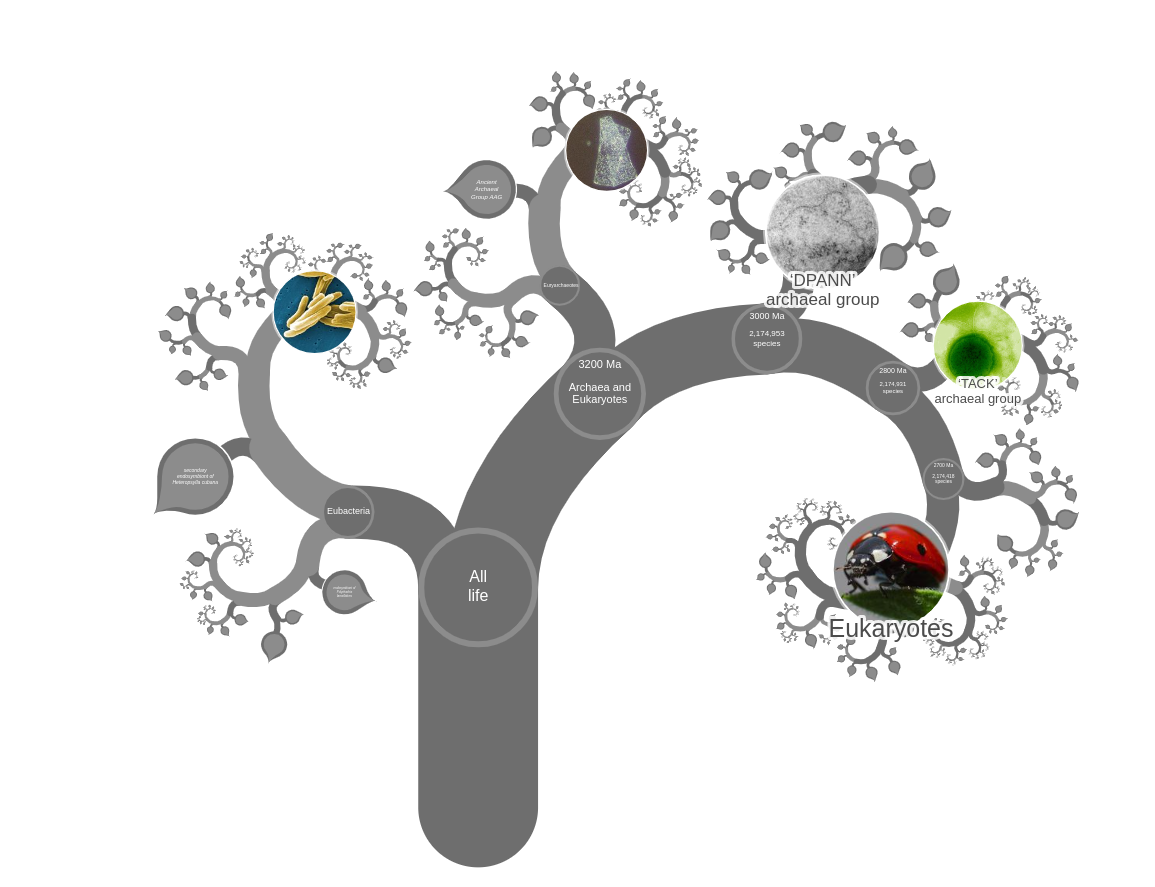
\includegraphics[width=0.45\textwidth]{figures/related_work/onezoom_overview}\label{fig:OneZoom_a}} 
	\hfill
	\subfigure[The view on OneZoom's tree when zoomed onto mammals. ]{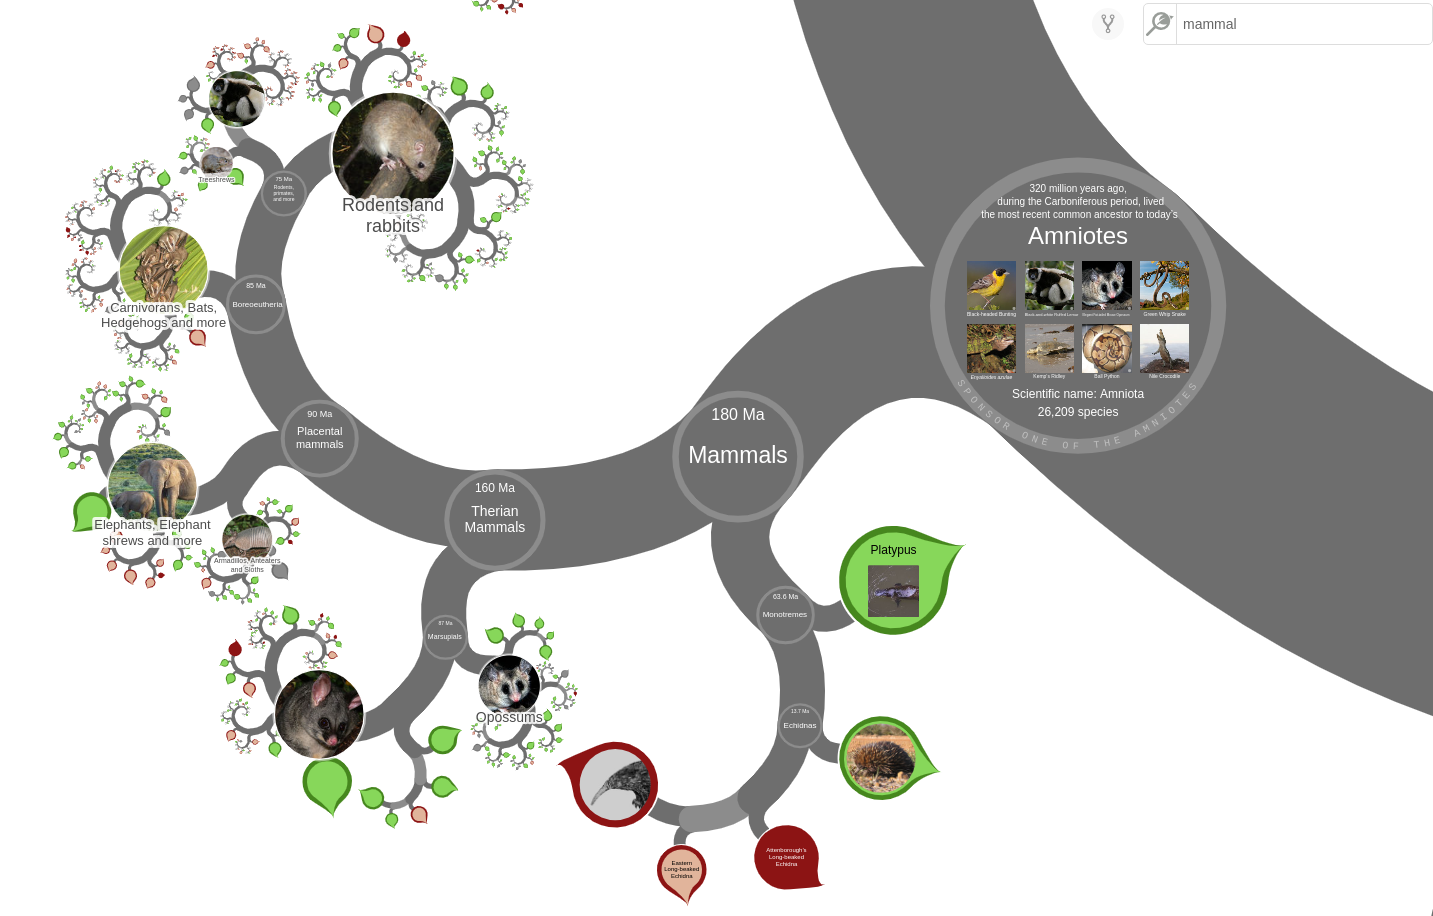
\includegraphics[width=0.45\textwidth]{figures/related_work/onezoom_mammal}\label{fig:OneZoom_b}} 
	\caption{Tree of life implementation in OneZoom. }
	\label{fig:OneZoom}
\end{figure}

The fractal design gives the tree a nice appearance, with leaves and nodes resembling the leaves and branches of an actual tree. General information such as pictures or earliest time of a node is also well packed in the interactive image. There is a reset button to return to the root, and a drop down list that provides links to the nodes along the path to root from the current position. These functions are convenient for navigation and similar functionality should be implemented in this thesis. It is claimed that all categorized organisms, which has a total amount of over two million, are included in the tree. Each species in the tree structure are incorporated with a phylogenetic classification, indicating that for a particular species represented by a leaf to reach the root, it visits all of the nodes representing each of its ancestor throughout the evolutionary history. Although how a certain organism evolved from the common ancestor of all life can be rigorously inspected, from the user experience's point of view, the tree is extremely deep. Apart from manually searching for a name, navigating to a desired location in this deep tree is mainly achieved by scrolling and dragging the item of interest to the center of the screen. This makes it difficult for viewers to relocate to a different section of the tree, or to gain an overview of where the current node or leaf sits in the entire tree of life. To reach the root (\ref{fig:OneZoom_a}) from mammal (\ref{fig:OneZoom_b}) while viewing its path, users need to scroll through all upper levels of the similar-looking spiral structures of the tree, which appears to be confusing. A similar tree of life is Lifemap (\url{http://lifemap.univ-lyon1.fr/explore.html}), which ameliorates the navigation difficulty by highlighting the ancestry path from root to an entry (Fig\ref{fig:lifemap}). However, due to the sheer depth of the tree, users still need to travel deep into the tree by scrolling. Rather than demonstrating the exact ancestral paths, the purpose of the tree for this project is to organize each species such that biodiversity can be viewed in an intuitive way. As a consequence, all entries can be organized in only the main taxonomic ranks, limiting the tree's depth to be eight and thus simplifying the navigation process. In addition, to avoid scrolling and dragging, the tree can take a fixed position, while where a node or leaf locates can be shown in a clickable breadcrumb structure that provides an overview of the whole tree. \\

\begin{figure}[h]
	\centering
	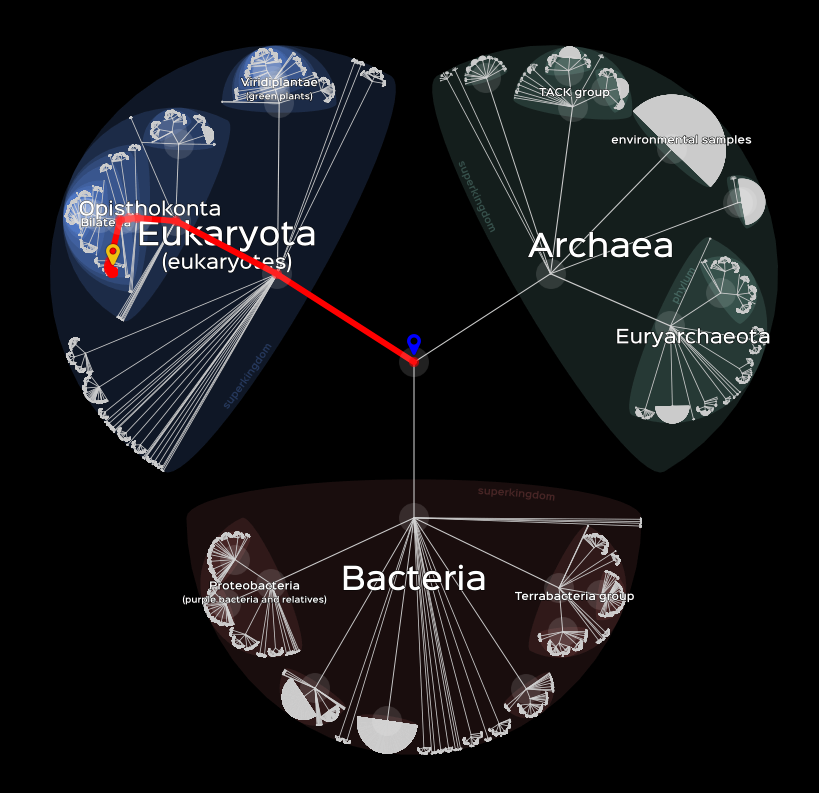
\includegraphics[width=0.5\textwidth]{figures/related_work/lifemap}
	\caption{Lifemap enables a "path from root" functionality that highlights the ancestry path from \textit{Homo sapiens} to the root. }
	\label{fig:lifemap}
\end{figure}

A much simplified version of tree of life is Evogeneao (\url{https://www.evogeneao.com/en/explore/tree-of-life-explorer}), which is intended for school education. As shown in Fig\ref{fig:evogeneao}, all species are grouped into clearly colored groups, which gives the viewers a direct and memorable visual impact. A similar design could be adapted in this project. With the tree of life arranged in a half circle that is labeled with time and a few iconic events, users could get a view of how life radiated from the common ancestor into great diversity, and how this process is affected by special events on the planet. Since only a small subset of all organisms are shown, the tree is small and can be entirely shown, thus always giving the audience an overview. However, this web application provides little possibility of exploration due to its limited options for interaction, as the main functionality is to show the common ancestor of two selected items (Fig\ref{fig:evogeneao_b}).

\begin{figure}[h]
	\centering
	\subfigure[The overview of Evogeneao's tree. ]{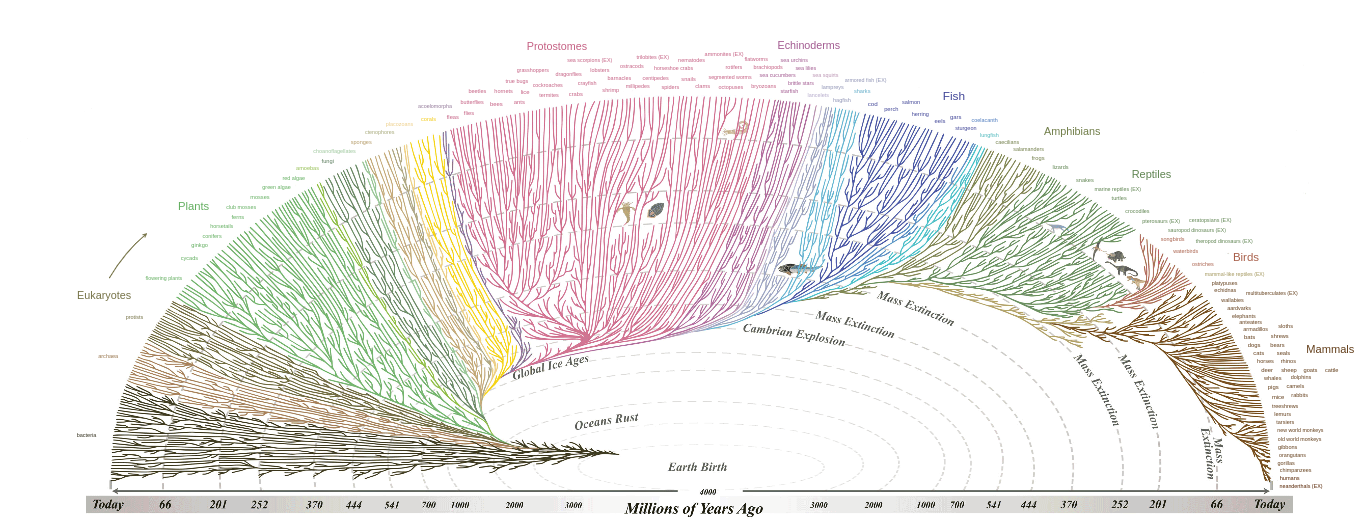
\includegraphics[width=0.45\textwidth]{figures/related_work/evogeneao_overview}\label{fig:evogeneao_a}} 
	\hfill
	\subfigure[The ancestral relationship between human and songbird. ]{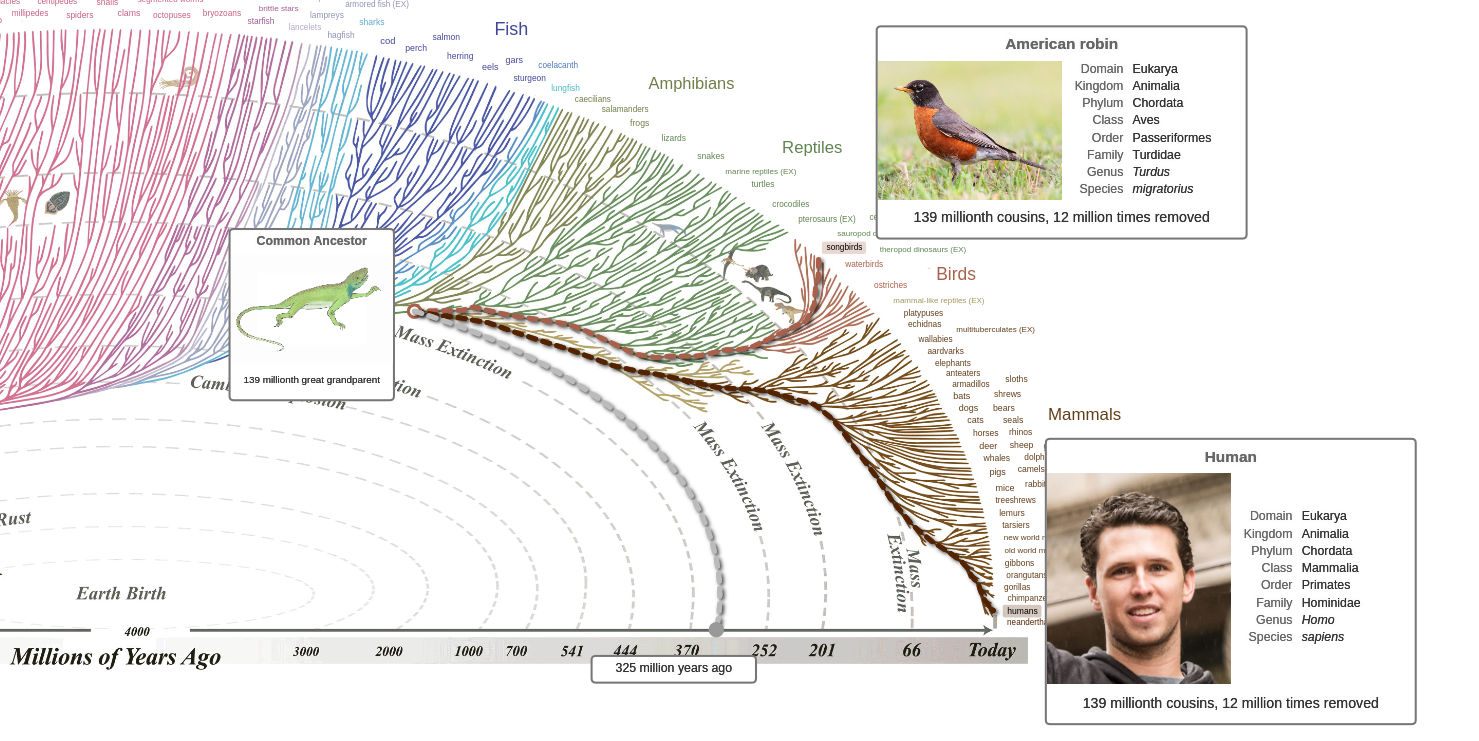
\includegraphics[width=0.45\textwidth]{figures/related_work/evogeneao_relationship}\label{fig:evogeneao_b}} 
	\caption{Tree of life implementation in iTOL. }
	\label{fig:iTOL}
\end{figure}

Finally, there are a wide variety of tree of life visualized for computational biologists. Such visualizations provide rich functionalities for bioinformatic analysis that are well beyond the need of general public and often take efforts to use. An example is iTOL (\url{https://itol.embl.de/itol.cgi},Fig\ref{fig:iTOL}). The design of arranging all leaves on the edge of a circle and all nodes in its interior utilizes space effectively, therefore can be adapted in our implementation. 

\begin{figure}[h]
	\centering
	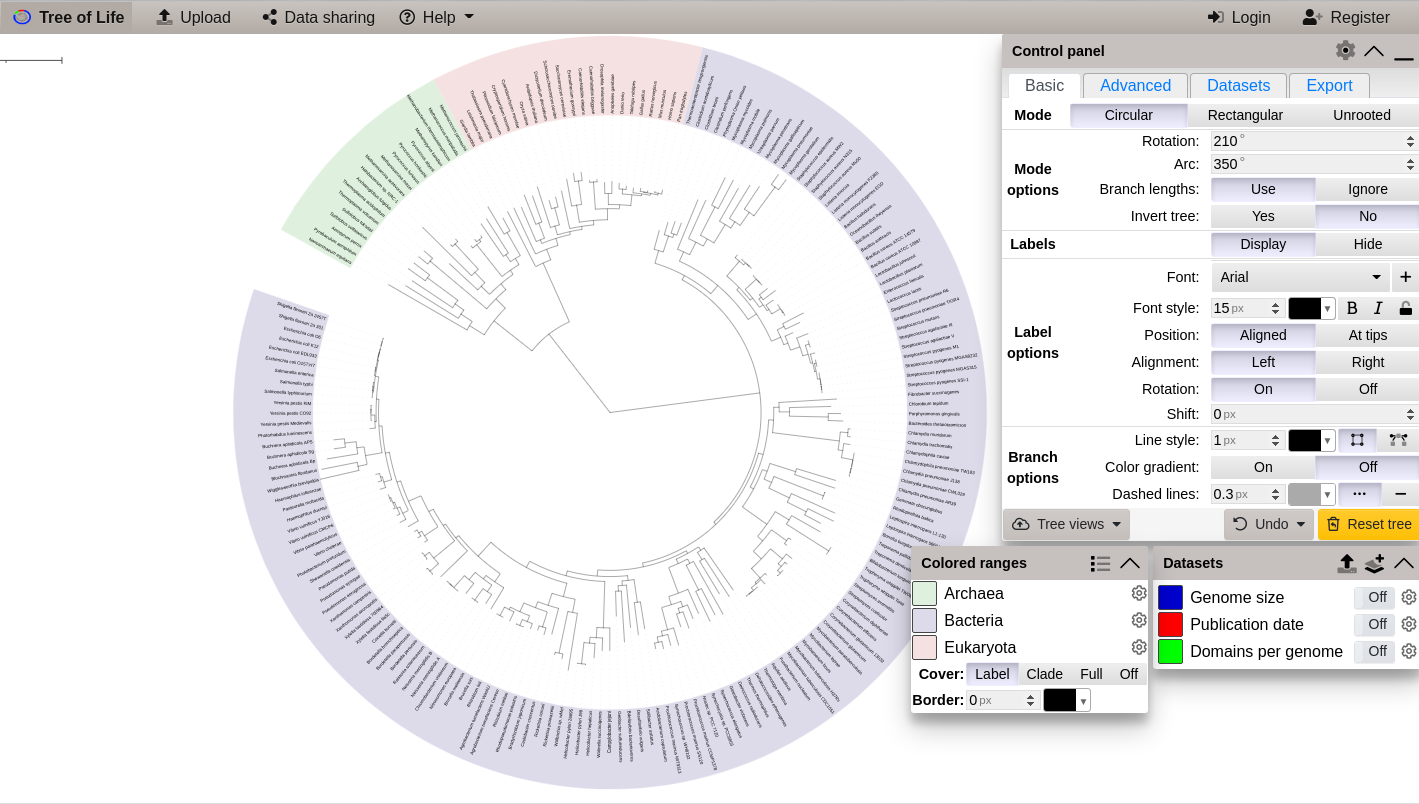
\includegraphics[width=0.5\textwidth]{figures/related_work/iTOL}
	\caption{Tree of life in iTOL. }
	\label{fig:iTOL}
\end{figure}

\section{Visualizations on tectonic shift}
\begin{figure}[h]
	\centering
	\subfigure[Tectonic shift visualized in Ancient Earth. ]{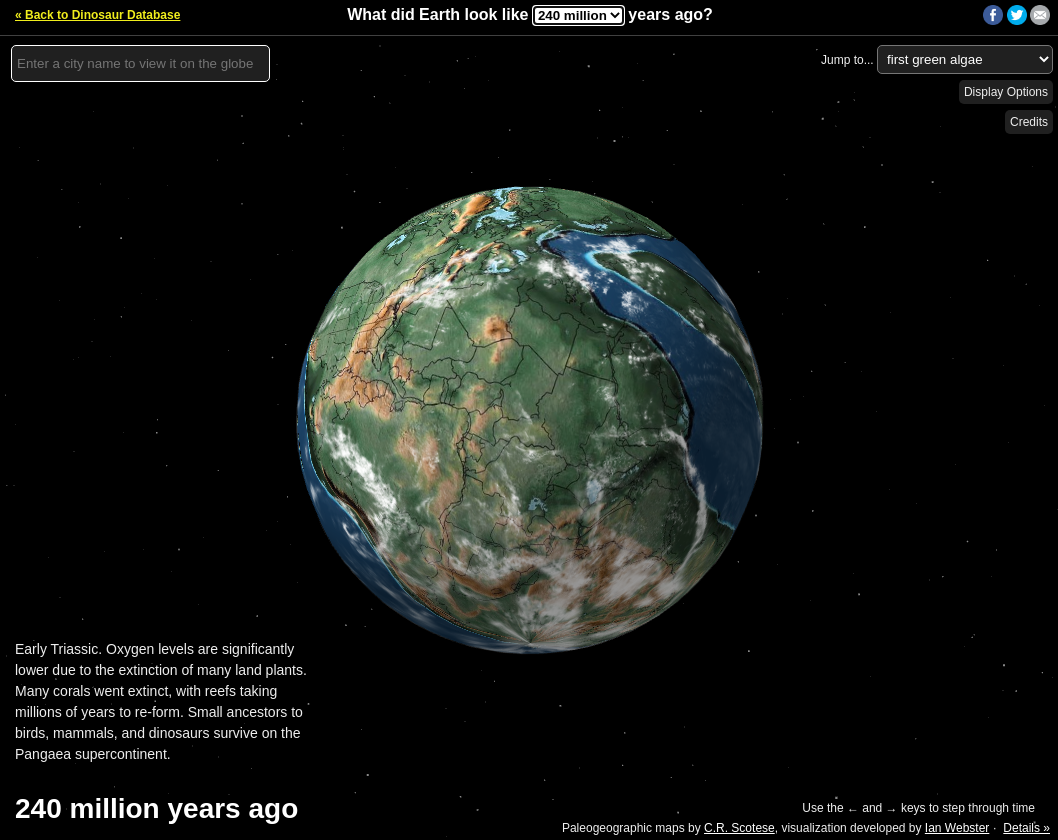
\includegraphics[width=0.45\textwidth]{figures/related_work/ancient_earth}\label{fig:ancient_earth}} 
	\hfill
	\subfigure[Tectonic shift visualized in Earth Viewer. ]{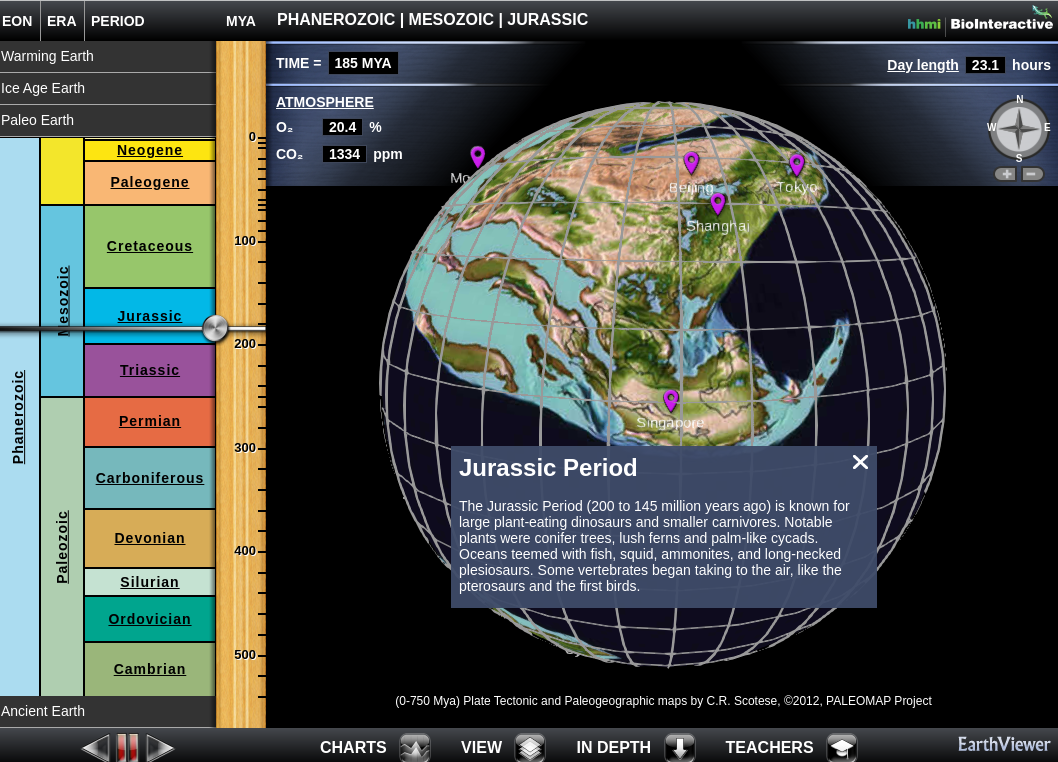
\includegraphics[width=0.45\textwidth]{figures/related_work/earth_viewer}\label{fig:earth_viewer}} 
	\caption{Example visualizations on tectonic shift. }
	\label{fig:tectonic_shift}
\end{figure}
Current project involves visualizing plate motions in various time period, since biodiversity information is shown on the world map during the select time period of interest. Two typical tectonic shift visualizations are Ancient Earth (\url{https://dinosaurpictures.org/ancient-earth#240}, Fig\ref{fig:ancient_earth}) and Earth Viewer (\url{https://www.biointeractive.org/classroom-resources/earthviewer}, Fig\ref{fig:earth_viewer}). Both of them show the coastlines of the continents at a select time point on a three-dimensional globe. Ancient Earth allows users to pick a particular time point from a list of options and search for the ancient location of a city. Earth Viewer provides more detailed information on geological time, and selectable time points are incremented at every five million years on the scroll bar. Time periods are organized in a hierarchical structure with names, which can be adapted in this project for easy navigation. When clicking on a time period, instead of directing the user to the selection, a pop-up window containing a brief introduction of the time period appears, which is counter-intuitive. An improvement is to show the earth at the middle of the selected time period upon clicking.

%=====================================================================
\chapter{Problem statement} \label{chp:problem_statement}
%=====================================================================
The data visualization project is divided into several sub-problems as follows.

\begin{itemize}
	\item \textbf{Data processing}
	\begin{itemize}
		\item Process the PBDB dataset to extract fossil records 
		\item Extract a tree of life from the taxonomy information of the fossil record 
		\item Trace the coordinates of each fossil record to ancient time
	\end{itemize} 
	\item \textbf{Database setup}: store the fossil data, coordinate data and the taxonomy data into a database
	\item \textbf{Back-end building}: enable data queries from the database upon users' request from the front-end 
	\item \textbf{Front-end building}: visualize interactive components for users to explore biodiversity through deep time
	\begin{itemize}
		\item A time component that lists ancient epochs that users can select
		\item A tree component that shows the tree of life constructed by the fossil records found in the selected time period, under the selected taxonomy. 
		\item A map component that shows the shape of the continents in the selected time period, and the locations of the fossil records that constitutes the tree of life in the above component.    
	\end{itemize} 
\end{itemize} 

%=====================================================================
\chapter{Technical solution} \label{chp:technical_solution}
%=====================================================================
\section{Overview}\label{sec:tec_overview}
This section explains the technical solutions to the problems stated in chapter \ref{chp:problem_statement}. To summarize, the project is divided into data processing in section \ref{sec:tec_data_processing}, database setup in section \ref{sec:tec_database_setup}, back-end development in section \ref{sec:tec_backend} and front-end development in section \ref{sec:tec_frontend}.

\section{Data processing} \label{sec:tec_data_processing}
\subsection{Fossil data parsing and processing} \label{subsec:fossil_data_processing}
PBDB dataset is used for both fossil data and tree data. The raw data consists of two csv files that contain 1240202 animal fossil records and 105918 plant fossil records, respectively. Since the two files share the same data attributes, the data is concatenated into one file. Only the attributes that are relevant to this project are kept, which is listed below.\\

\noindent Extracted attributes in the PBDB dataset:
\begin{itemize}
	\item \textit{occurrence\_no}: a unique ID code for a fossil record
	\item \textit{accepted\_name}: the accepted name of a fossil record
	\item \textit{accepted\_rank}: the taxonomic rank in which the accepted\_name belongs to 
	\item \textit{phylum}: the phylum name of the fossil record
	\item \textit{class}: the class name of the fossil record
	\item \textit{order}: the order name of the fossil record
	\item \textit{family}: the family name of the fossil record
	\item \textit{genus}: the genus name of the fossil record
	\item \textit{max\_ma}: the oldest estimated time of the fossil record, in million years
	\item \textit{min\_ma}: the earliest estimated time of the fossil record, in million years
	\item \textit{lng}: the longitude of the fossil record's found location 
	\item \textit{lat}: the latitude of the fossil record's found location 
	
\end{itemize}

In addition, there are four additional attributes are appended to the current data frame, for the construction of tree of life in the next step. \\

\noindent Computed attributes added to the PBDB data frame:
\begin{itemize}
	\item \textit{kingdom}: the kingdom name of the fossil record
	\item \textit{path\_from\_root}: a comma separated string indicating the taxonomic path from a fossil record's name to its root
	\item \textit{name}: the taxon name of the fossil record on the lowest taxonomic rank
	\item \textit{unique\_name}: the unique name of the fossil record

\end{itemize}


Firstly, the kingdom of Animalia and Plantae is assigned to each fossil record, depending on whether it is originated from the animal or plant file, respectively. The domain name is not required, since all records are either an animal or a plant, both of which reside in the domain of Eukaryota. \\

The attribute \emph{path\_from\_root} is a comma separated string of taxonomic names in the order of the highest taxonomic rank (domain) to the lowest taxonomic rank with an available name. Note that the dataset does not have an attribute named \emph{species}. Instead, when the species or subspecies name of a record is available, the record would have the attribute \emph{accepted\_rank} labeled as \emph{species} or \emph{subspecies}, and the name is found in the attribute \emph{accepted\_name}. For each fossil record, we iterate from the highest rank, domain, to the lowest rank, species, while appending the name on each rank level to the \emph{path\_from\_root} string. The process terminates when encountering an empty field, or when reaching to the species level. As a consequence, when a record is missing a name on a certain taxonomic rank, its \emph{path\_from\_root} only describes up to the rank above the missing rank to prevent ambiguity of a path, even though the record may have names available below the missing rank. Extra knowledge in taxonomy is needed to retrieve the missing names. Therefore, this challenge is beyond the scope of the current project. \\

The attribute \emph{name} is the name on the lowest rank from \emph{path\_from\_root}, namely, the string after the last comma. This attribute is required to generate \emph{unique\_name}, which serves as an unique identifier of an entry on the to-be-constructed tree of life. The value of \emph{unique\_name} is equivalent to \emph{name}, when \emph{name} is unique. Otherwise, it uses the value of \emph{path\_from\_root}.

\subsection{Generation of tree from taxonomy} \label{subsec:tree_generation}
The fossil records can be organized in a tree of life that is computed using the taxonomic information from the processed PBDB dataset. The resulted flattened tree structure has the following attribute:

\begin{itemize}
	\item \textit{unique\_name}: the unique name of a node or leaf in the tree
	\item \textit{path\_from\_root}: a comma separated string indicating the taxonomic path from a node's or leaf's name to its root
	\item \textit{parent}: the unique name of the entry's parent
	\item \textit{children}: a list of the unique names of the entry's children
\end{itemize}

The tree data contains all nodes and leaves of the tree of life formed by the taxonomy of the fossil records. We initialize the tree data frame by extracting all the unique \emph{path\_from\_root} values from the processed fossil data from section \ref{subsec:fossil_data_processing}. However, there are more nodes to include in the tree. For each entry in the tree represented by its \emph{path\_from\_root}, we must also include each of the upstream ancestor in the tree. For instance, when the item "a,b,c,d" is included, its ancestors "a,b,c", "a,b" and "a" are also present in the tree. Therefore, the next step is to iterate through each of the unique \emph{path\_from\_root} and append the additional nodes. \\

The next steps are to append the \emph{unique\_name}, \emph{parent} and \emph{children} values for each \emph{path\_from\_root}. Similar to section \ref{subsec:fossil_data_processing}, we compute \emph{unique\_name} from \emph{path\_from\_root}, by firstly extracting \emph{name}, the name on the lowest rank, and assign either \emph{name} to \emph{unique\_name} if \emph{name} is unique, or assign \emph{path\_from\_root} to \emph{unique\_name} if otherwise. \\

The attribute \emph{parent} can be obtained from slicing the \emph{path\_from\_root} from start to its last comma (the \emph{path\_from\_root} value of its parent), and assigning the corresponding \emph{unique\_name} value to \emph{parent}. Lastly, we iterate through each \emph{unique\_name} and append the list of \emph{unique\_name} values of all the items whose \emph{parent} equals the current \emph{unique\_name} in each iteration.

\subsection{Conversion of modern coordinates to ancient coordinates} \label{subsec:coordinate_conversion}
To convert coastlines and fossil locations to ancient time, we use the model proposed by Matthew. \\

Geological time period data is hierarchical. The hierarchy contains five layers, with the top most layer Phanerozoic. A time period in a deeper layer is shorter. The ancient year that the coordinates are translated into is the middle value rounded to the integer, between the start and end years of the smallest time period, i.e., layer five. 

\section{Database setup} \label{sec:tec_database_setup}


\section{Back-end development} \label{sec:tec_backend}


\section{Front-end development} \label{sec:tec_frontend}


%=====================================================================
\chapter{Implementation} \label{chp:implementation}
%=====================================================================
\section{Code structure} \label{sec:implementation_code_structure}
\section{Data process stacks}\label{sec:implementation_data_processing}
\section{Web development stacks}\label{sec:implementation_web_development}

%=====================================================================
\chapter{Results} \label{chp:results}
%=====================================================================
\section{Data analysis} \label{sec:result_data_analysis}
\subsection{fossil data} \label{subsec:data_analysis_fossil}
\subsection{tree data} \label{subsec:data_analysis_tree}

\section{Data visualization} \label{sec:result_data_visualization}
\subsection{Time selector component} \label{subsec:data_visualization_time}
\subsection{Map component} \label{subsec:data_visualization_map}
\subsection{Tree component} \label{subsec:data_visualization_component}
%=====================================================================
\chapter{Conclusion} \label{chp:discussion_conclusion}
%=====================================================================



\section{Limitations and Future Work}

%=====================================================================
\chapter*{Acknowledgements}
%=====================================================================


\bibliographystyle{alpha}
\bibliography{references}

\listoffigures
\listoftables
%=====================================================================
\appendix
\chapter{Appendix}
The appendix of this thesis is stored on a DVD which is attached to the end of the printed document. It includes the follow items: 
\begin{enumerate}
    \item \textbf{code/} The full application code. 
    \item \textbf{report/} The complete report as latex source
    \item \textbf{Masterarbeit.pdf} This report in its digital version
    \item{Abstract.txt} The abstract to this thesis in English
    \item {Zusfsg.txt} The abstract to this thesis in German
\end{enumerate}

%=====================================================================
\end{document}

